\documentclass{article}
% Hyperreferences
\usepackage{hyperref}
% Margins
\usepackage[top=35mm,bottom=35mm,left=25mm,right=25mm]{geometry}
% Graphics and images
\usepackage{graphicx}
\graphicspath{{./images/}}
% Encodings (to render letters with diacritics and special characters)
\usepackage[utf8]{inputenc}
% Language
\usepackage[english]{babel}
% Section pagebreaks
\usepackage{titlesec}
\newcommand{\sectionbreak}{\clearpage}
\newcommand{\sectionnobreak}{% for when I want a section that does not break
  \global\toggletrue{afterpart}%
  \section
}
% Source code
\usepackage{listings}
\usepackage{xcolor}
\renewcommand{\lstlistingname}{File}
\lstset{
    frame=tb, % draw frame at top and bottom of the code
    tabsize=4, % tab space width
    numbers=left, % display line numbers on the left
	showstringspaces=false, % don't mark spaces in strings    
    commentstyle=\color{green}, % comment color
    keywordstyle=\color{blue}, % keyword color
    stringstyle=\color{red} % string color
}
\lstdefinelanguage{Maxima}{
	keywords={log,jacobian,determinant,subst},
	sensitive=true,
	comment=[n][\itshape]{/*}{*/}
}
% Tables with bold rows
\usepackage{tabularx}
\newcommand\setrow[1]{\gdef\rowmac{#1}#1\ignorespaces}
\newcommand\clearrow{\global\let\rowmac\relax}
\clearrow
% Math stuff
\usepackage[mathscr]{euscript}
\usepackage{amsmath,amssymb}
\usepackage{mathtools}
\usepackage{enumitem}
\newcommand{\expnumber}[2]{{#1}\mathrm{e}{#2}} % scientific notation
% Definitions, theorems, remarks,...
\usepackage{amsthm}
\newtheorem{definition}{Definition}[section]
\newtheorem{theorem}{Theorem}[section]
\newtheorem{corollary}{Corollary}[theorem]
\newtheorem{lemma}[theorem]{Lemma}
\renewcommand\qedsymbol{$\blacksquare$}
\theoremstyle{remark}
\newtheorem*{remark}{Remark}
% Contents title
\addto\captionsenglish{\renewcommand*\contentsname{Table of contents}}
% Headers and footers
\usepackage{fancyhdr}
\pagestyle{fancyplain}
\fancyhf{}
\lhead{ \fancyplain{}{LabWars - Final report (LCOM 2019/20)}}
\lfoot{ \fancyplain{}{T5G03}}
\rfoot{ \fancyplain{}{\thepage} }
%
\newcommand{\email}[1]{
{\texttt{\href{mailto:#1}{#1}} }
}
\newcommand{\role}[1]{
\begin{tabular}{l l}
	\begin{minipage}[t]{30mm} \textbf{Roles} \end{minipage} &
	\begin{minipage}[t]{125mm} #1 \end{minipage}
\end{tabular}\\
}
\newcommand{\func}[1]{
\begin{tabular}{l l}
	\begin{minipage}[t]{30mm} \textbf{Functionalities} \end{minipage} &
	\begin{minipage}[t]{125mm} #1 \end{minipage}
\end{tabular}\\
}
% Metadata
\title{\Huge LabWars \\ \Large Final report \\ \vspace*{4pt} \large LCOM 2019/20}
\author{
T5G03\\
\begin{tabular}{r l}
	\email{up201806429@fe.up.pt} & Diogo Miguel Ferreira Rodrigues        \\
	\email{up201806554@fe.up.pt} & Telmo Alexandre Espirito Santo Baptista
\end{tabular}
}
\date{06/01/2020}
% Document
\begin{document}
%\begingroup
	\maketitle
%	\let\clearpage\relax
%	\setcounter{tocdepth}{2}
	\tableofcontents
%\endgroup
\section{User instructions}
\subsection{Main menu}
On startup, users are greeted by a \texttt{Loading...} message, briefly followed by the main screen.
\begin{center} 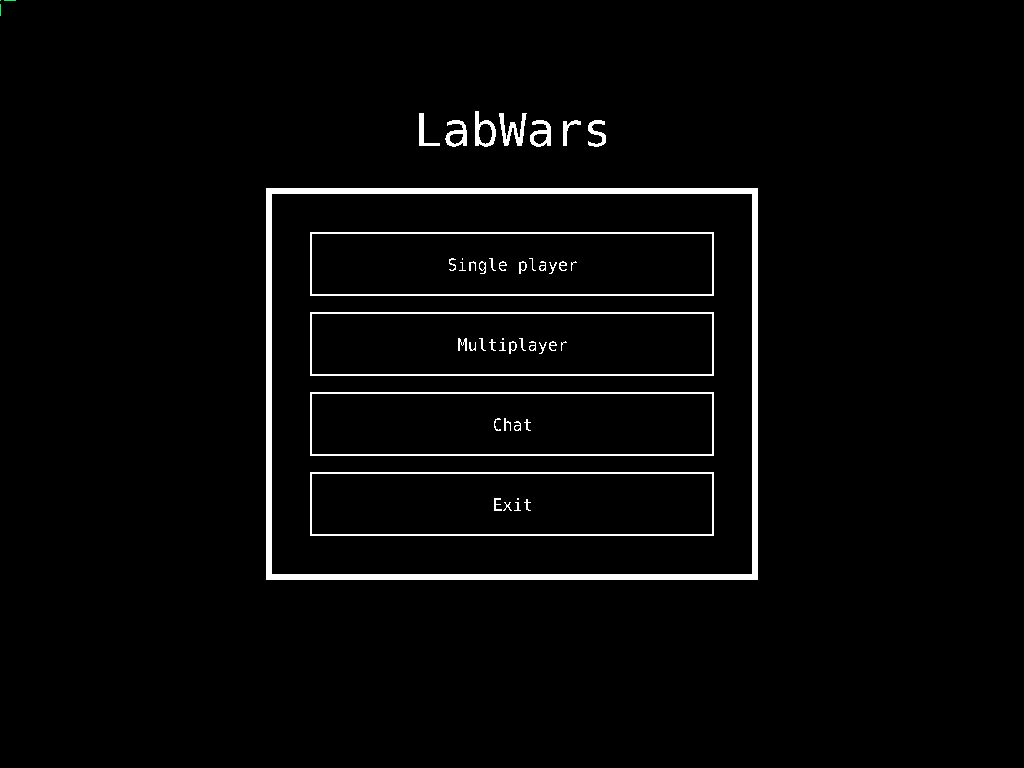
\includegraphics[scale=0.45]{main_menu} \end{center}

\subsection{Chat}
This chat tool was initially designed as a simple, text mode, test communication between different machines. We have however decided to include it as a functionality in the project for a number of reasons:
\begin{enumerate}
	\item It was easy to develop the graphical part and integrate in the project.
	\item Having a friendly functionality that uses the communication modules allows for faster debugging; in case the computers are not properly connected, or if during development something stops working we can immediately check if the communication modules also stopped working.
	\item It served as a minimal insurance that our project would integrate the communication modules, in case we could not implement multiplayer mode.
	\item It is a useful feature.
\end{enumerate}

\section{Project status}
Hey
\section{Code organization/structure}
Hey
\section{Implementation details}
Hey
\section{Conclusions}
Hey
\end{document}
